
\section{Rufzeichen}
\label{section:rufzeichen}
\begin{frame}%STARTCONTENT

\frametitle{Rufzeichen}
\begin{columns}
    \begin{column}{0.48\textwidth}
    
\begin{figure}
    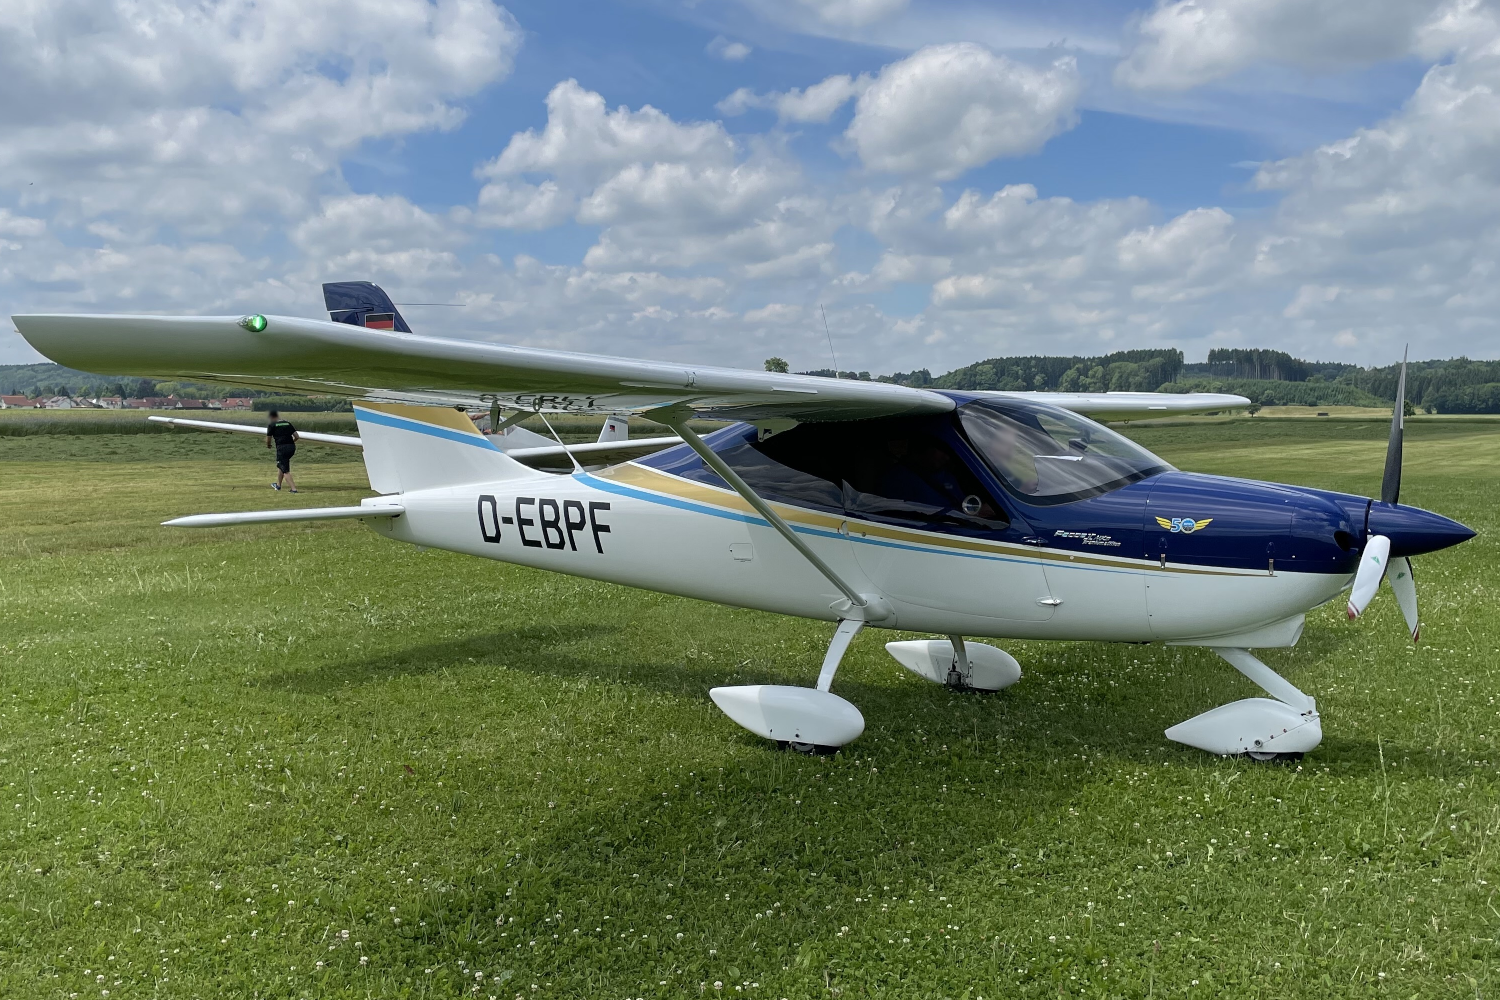
\includegraphics[width=0.85\textwidth]{foto/167}
    \caption{\scriptsize Flugzeug mit dem Rufzeichen DEBPF}
    \label{rufzeichen_flugzeug}
\end{figure}

    \end{column}
   \begin{column}{0.48\textwidth}
       \begin{itemize}
  \item Funkstationen verwenden Rufzeichen, um sich zu identifizieren
  \item Folge von Buchstaben und Ziffern
  \item Jedes mit Funk ausgerüstete Flugzeug und Schiff hat ein Rufzeichen
  \end{itemize}

   \end{column}
\end{columns}

\end{frame}

\begin{frame}
\frametitle{Amateurfunkrufzeichen}
\begin{itemize}
  \item Persönliches Rufzeichen wird zugeteilt
  \item Weltweit eindeutig
  \item Muss am Anfang und Ende jeder Verbindung genannt werden
  \item Und alle 10 Minuten bei längeren Verbindungen
  \end{itemize}
\end{frame}

\begin{frame}
\only<1>{
\begin{QQuestion}{VD207}{Woran erkennt man eine Amateurfunkstelle im Funkbetrieb?}{Am Amateurfunkrufzeichen}
{Am benutzten Frequenzbereich}
{An der verwendeten Sendeart}
{An der Modulation}
\end{QQuestion}

}
\only<2>{
\begin{QQuestion}{VD207}{Woran erkennt man eine Amateurfunkstelle im Funkbetrieb?}{\textbf{\textcolor{DARCgreen}{Am Amateurfunkrufzeichen}}}
{Am benutzten Frequenzbereich}
{An der verwendeten Sendeart}
{An der Modulation}
\end{QQuestion}

}
\end{frame}

\begin{frame}
\only<1>{
\begin{QQuestion}{VD205}{Wann muss der Funkamateur sein Rufzeichen nennen?}{Mindestens alle 15~Minuten während einer Funkverbindung}
{Auf Verlangen einer anderen am Funkverkehr beteiligten Funkstelle}
{Am Anfang und am Ende jeder Funkverbindung sowie mindestens alle 10~Minuten}
{Spätestens 5~Minuten nach einer ununterbrochenen Aussendung}
\end{QQuestion}

}
\only<2>{
\begin{QQuestion}{VD205}{Wann muss der Funkamateur sein Rufzeichen nennen?}{Mindestens alle 15~Minuten während einer Funkverbindung}
{Auf Verlangen einer anderen am Funkverkehr beteiligten Funkstelle}
{\textbf{\textcolor{DARCgreen}{Am Anfang und am Ende jeder Funkverbindung sowie mindestens alle 10~Minuten}}}
{Spätestens 5~Minuten nach einer ununterbrochenen Aussendung}
\end{QQuestion}

}
\end{frame}%ENDCONTENT
